%%%%%%%%%%%%%%%%%%%%%%%%%%%%%%%%%%%%%%%%%%%%%%%%%%%%%%%%%%%%%%%%%%%%%%%%%%%%%%%%
% detector_performance.tex: Chapter on Detector Performance:
%%%%%%%%%%%%%%%%%%%%%%%%%%%%%%%%%%%%%%%%%%%%%%%%%%%%%%%%%%%%%%%%%%%%%%%%%%%%%%%%
\chapter{Detector Performance}
\label{detector_performance_chapter}
%%%%%%%%%%%%%%%%%%%%%%%%%%%%%%%%%%%%%%%%%%%%%%%%%%%%%%%%%%%%%%%%%%%%%%%%%%%%%%%%

%%%%%%%%%%%%%%%%%%%%%%%%%%%%%%%%%%%%%%%%%%%%%%%%%%%%%%%%%%%%%%%%%%%%%%%%%%%%%%%%
% Detector Yield 
%%%%%%%%%%%%%%%%%%%%%%%%%%%%%%%%%%%%%%%%%%%%%%%%%%%%%%%%%%%%%%%%%%%%%%%%%%%%%%%%
\section{Detector Yield}
\label{sec:yield}
%%%%%%%%%%%%%%%%%%%%%%%%%%%%%%%%%%%%%%%%%%%%%%%%%%%%%%%%%%%%%%%%%%%%%%%%%%%%%%%%


You need to say \ac{EBEX} and \ac{SQUID} before the table ...

\begin{table}[ht!]
\begin{center}
\begin{tabular}{l|c|c|c|c}
  & 150~GHz & 250~GHz & 410~GHz & Total \\
\hline Total number of bolometers on focal planes & 1120 & 560 & 280 & 1960 \\
\hline Able to read out with \ac{EBEX} electronics & 992 & 496 & 254 & 1742 \\
\hline Passed warm electrical \& visual inspections & 908 & 455 & 232 & 1595 \\
\hline Resistor \& dark \ac{SQUID} channels excluded & 861 & 447 & 213 & 1521 \\
\hline Detectors appearing in .8~K network analysis & 805 & 430 & 187 & 1422 \\
\hline Excluding SQUID failures & 773 & 414 & 155 & 1342 \\
\hline Poor performing detectors removed & 676 & 371 & 133 & 1180 \\
\hline Detectors with successful flight IV curves & 504 & 342 & 109 & 955 \\
% not including eccosorb/dark 492 & 317 & 92 & \
\hline
\end{tabular}
\end{center}
\caption{The detector yield broken down by observation frequency band, 150, 250, and 410~GHz, as well as the total number of detectors. Each row of the table accounts for detector loss.}
\label{yield_table}
\end{table}

\TAB\ref{yield_table} provides an accounting of \ac{EBEX} detector loss as a function of observation frequency band, as well as the total sum for the experiment.
Each silicon wafer, regardless of observation frequency band, had 140 bolometers. %and one alignment mark for the curious/pedantic
The 150 and 250~GHz wafers were coupled to \ac{LC} boards around the perimeter of the focal plane. These edge \ac{LC} boards each had 125 readout channels, 124 of which were connected to bolometers.  
The 410~GHz wafers were in the center of each focal plane and had central \ac{LC} boards in the space just behind the wafer. The central \ac{LC} boards each had 128 readout channels, 127 of which were connected to bolometers. %(because of the alignment mark). 
The first two rows of the table give the total number of bolometers flown and the total number of bolometers the electronics were capable of reading out. 

At room temperature, the wafers were inspected visually and each bolometer was tested for electrical continuity. 
The visual inspection was done under a microscope and, for example, sometimes revealed incomplete etching evidenced by a column of material from the \ac{TES} to the silicon. 
This was noted as a thermal short and such a detector was not electrically biased. 
For the electrical inspection, we measured the resistance by either probing directly across the wafer bond pads or by probing the leads on the \ac{LC} boards. 
The first method was done in the fabrication clean room and the second method was done after the wafer had been shipped, mounted, and wirebonded to its \ac{LC} board. 
The resistance reading was dominated by the room temperature resistance of the niobium leads. 
The electrical inspection could not identify a short across the \ac{TES} because the typical room temperature resistance of the \ac{TES} was a few ohms, much less than the tens of kiloohms of the niobium leads. 
The electrical inspection did, however, identify which \ac{TES} or leads did not make a complete electrical connection, i.e. were open. 
The warm visual and electrical inspection provided an upper limit of the wafer's yield because the open and thermally shorted detectors were guaranteed not to work, see the third row of \TAB\ref{yield_table}. 

For flight, each wafer had two bolometers replaced by 1~ohm resistors for monitoring read out electronic noise up to the \ac{LC} board, one channel at a low bias frequency and the other channel at a high bias frequency. 
Three \ac{SQUID}s were not attached to bolometer combs due to opens in the microstrips. These combs were modified to monitor read out electronic noise up to the \ac{SQUID}. See \TAB\ref{yield_table}, row 4. 

%
%Upon cooling the wafer, there are wired detector channels with a reasonable room temperature resistance, yet they do not appear in the network analysis, see \TAB\ref{yield_table}, row 5. Five \ac{SQUID}s failed to operate during flight, see \TAB\ref{yield_table}, row 6 for the yield after the \ac{SQUID} failures. 
%Once a wafer has been characterized in a dark cryostat, the detectors which degrade the noise performance of their comb are identified and their wirebonds are removed, see \TAB\ref{yield_table}, row 7. 
%%Occasionally, upon cooling a wafer a second time, additional detectors go missing from the network analysis. (And some detectors re-appear ... presumably due to poor quality wirebond connections.) See \TAB\ref{yield_table}, line "Survived \ac{EBEX} cooldown and plucking." \comred{remove word plucking and remove bad actor, replace with more clear description. no need to mention reappearances since they seldom happen and we only have conjectures as to why?}
%Finally, at float altitude, IV curves are performed and the total number of successful curves is reported in \TAB\ref{yield_table}, line 8. The losses between row 7 and row 8 are due to detectors being saturated or failing to transition. %(though typically they also failed to turn around during the characterization measurements, the loss isn't counted until flight because there was some hope they might work) or the IV curve exhibiting strange behaviour (e.g. a jump in the current reading). \comred{ben showed pv curve, but not iv curve. maybe just call it a pv curve and refer to detector fab section? NO. with reorganization, first mention of iv/pv curve comes after this table ??}
%
%
%%%%%%%%%%%%%%%%%%%%%%%%%%%%%%%%%%%%%%%%%%%%%%%%%%%%%%%%%%%%%%%%%%%%%%%%%%%%%%%%%
%% Loop Gain Calculation {{{
%%%%%%%%%%%%%%%%%%%%%%%%%%%%%%%%%%%%%%%%%%%%%%%%%%%%%%%%%%%%%%%%%%%%%%%%%%%%%%%%%
%\section{Detector Loop Gain}
%\label{sec:loop_gain}
%%%%%%%%%%%%%%%%%%%%%%%%%%%%%%%%%%%%%%%%%%%%%%%%%%%%%%%%%%%%%%%%%%%%%%%%%%%%%%%%%
%
%loop gain blah blah blah
%
%\begin{figure}[htbp]
%\begin{center}
%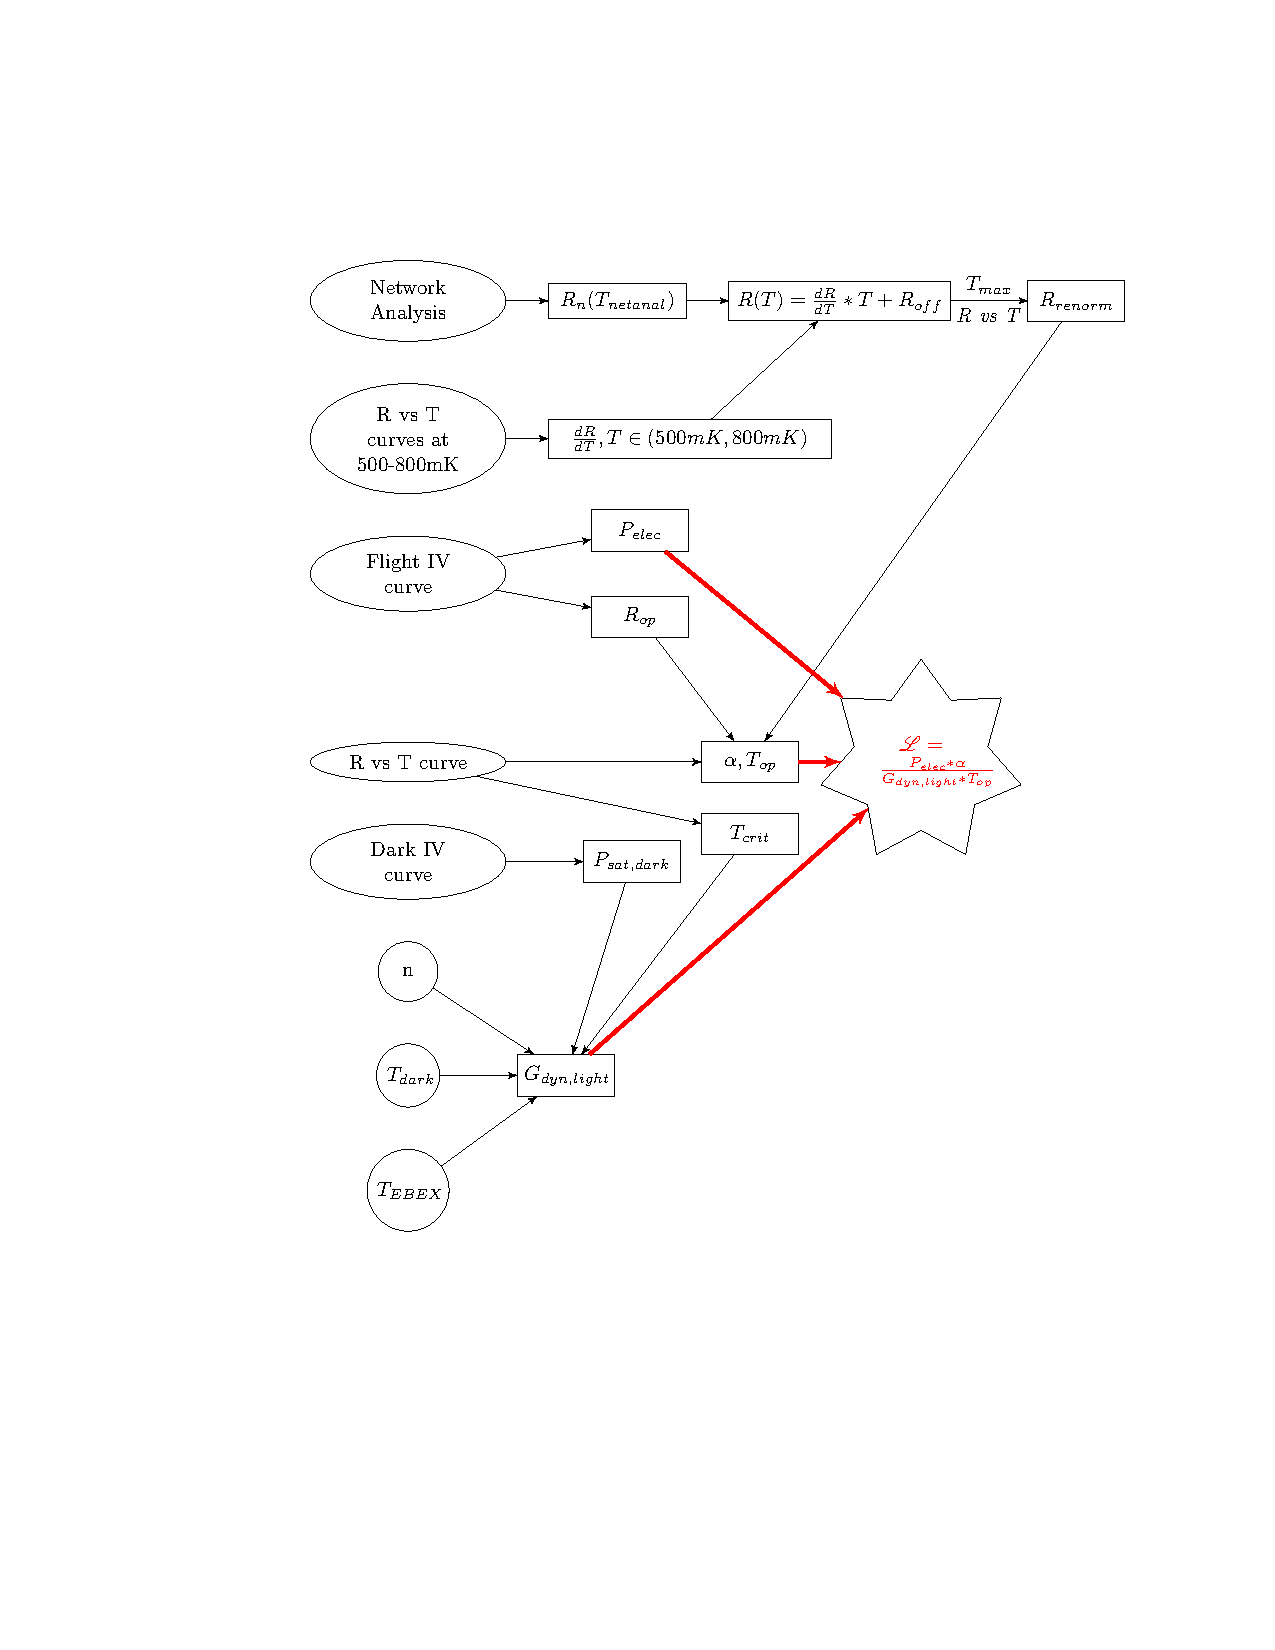
\includegraphics[width=1.0 \textwidth]{figures/loopgain_flowchart.pdf}
%\caption{Loop gain calculation flow chart}
%\label{fig:loopgain_flow}
%\end{center}
%\end{figure}
%
%The slope of the Resistance vs Temperature curve for 410-18 between .550 and .800~K was $0.29\pm0.05 \Omega/K$. 
%
%\begin{figure}[htbp]
%\begin{center}
%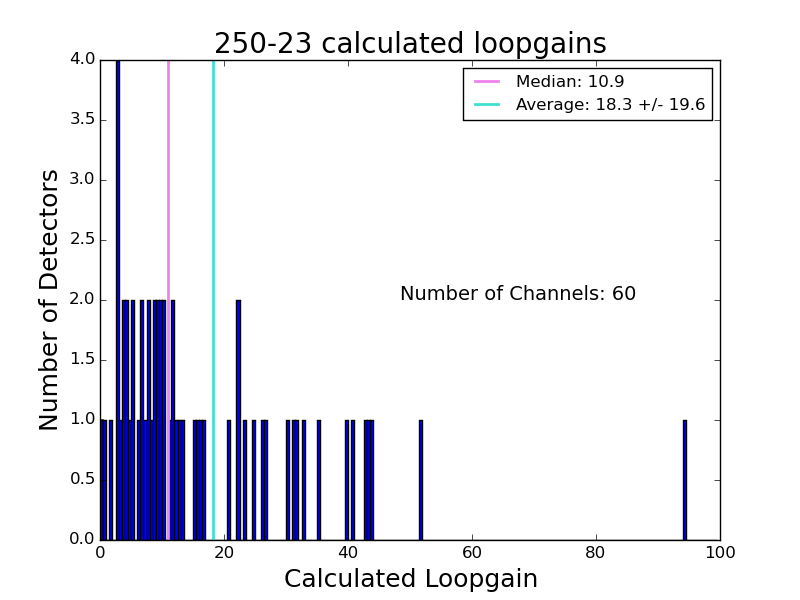
\includegraphics[width=0.5 \textwidth]{figures/250-23_loopgains_calculated_tuning3.png}
%\caption{Loop gains calculated for 250-23 for tuning3.}
%\label{fig:loopgain_calc_hist}
%\end{center}
%\end{figure}
%
%\begin{figure}[htbp]
%\begin{center}
%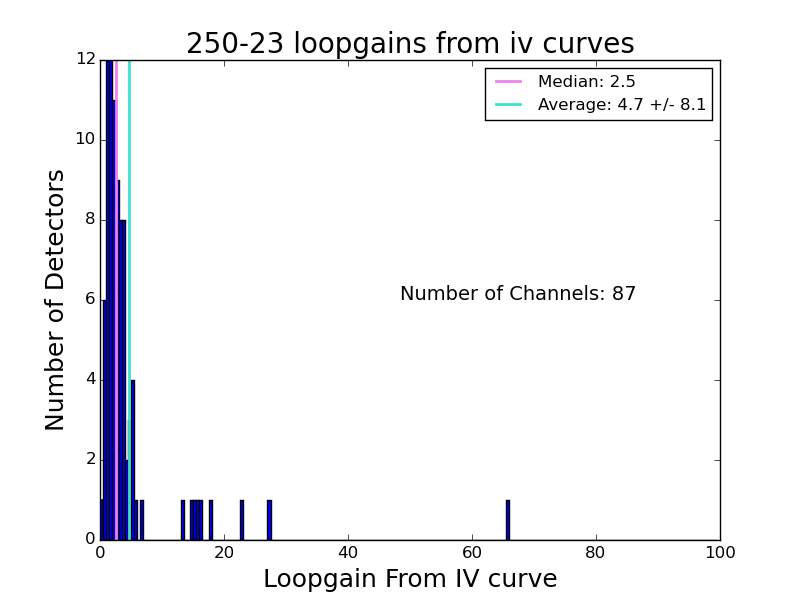
\includegraphics[width=0.5 \textwidth]{figures/250-23_loopgains_from_iv_tuning3.png}
%\caption{Loop gains estimated from each 250-23 bolometer's flight IV curve for tuning3.}
%\label{fig:loopgain_from_iv_hist}
%\end{center}
%\end{figure}
%
%
%%%%%%%%%%%%%%%%%%%%%%%%%%%%%%%%%%%%%%%%%%%%%%%%%%%%%%%%%%%%%%%%%%%%%%%%%%%%%%}}}
%
%
%
%%%%%%%%%%%%%%%%%%%%%%%%%%%%%%%%%%%%%%%%%%%%%%%%%%%%%%%%%%%%%%%%%%%%%%%%%%%%%%%%%
%% Detector Sensitivity {{{
%%%%%%%%%%%%%%%%%%%%%%%%%%%%%%%%%%%%%%%%%%%%%%%%%%%%%%%%%%%%%%%%%%%%%%%%%%%%%%%%%
%\section{Detector Sensitivity}
%\label{sensitivity}
%%%%%%%%%%%%%%%%%%%%%%%%%%%%%%%%%%%%%%%%%%%%%%%%%%%%%%%%%%%%%%%%%%%%%%%%%%%%%%%%%
%
%There are four units we use when measuring the detector noise equivalent power: ADC counts, Amps, Watts at the detector, and Watts on the sky. The total detector noise is recorded in ADC counts by the DfMUX boards. The predictions for the contributions of the current noise terms (Johnson and Readout) are naturally in units of Amps and the predictions for the contributions of the power noise terms (photon and phonon) are naturally in units of Watts at the detector. We also use each detector's calibration map of RCW38 to get a conversion from ADC counts to power on the sky in Watts.
%
%\begin{longtable}{| l | l | l |}
%\caption{Noise Equivalent Power, Unit Conversions} \label{NEP_table} \\
%  \hline
%  Measured Noise & Photon and Phonon Noise & Johnson and Readout Noise \\ \hline
%  $\big( \frac{\textbf{cts}^2}{\textbf{Hz}} \big)$ & $\big( \frac{W^2}{Hz} \big) \times \big( \frac{\text{cts}}{A_{sq}} \big) ^2 \times \big( S_I \big) ^2$ & $\big( \frac{A^2}{Hz} \big) \times \big( \frac{\text{cts}}{A_{sq}} \big) ^2 $ \\ \hline
%  $\big( \frac{\text{cts}^2}{\text{Hz}} \big) \times \big( \frac{A_{sq}}{\text{cts}} \big) ^2 $ & $\big( \frac{W^2}{Hz} \big) \times \big( S_I \big) ^2$ & $\big( \frac{\textbf{A}^2}{\textbf{Hz}} \big)$ \\ \hline
%  $\big( \frac{\text{cts}^2}{\text{Hz}} \big) \times \big( \frac{A_{sq}}{\text{cts}} \big) ^2 \times \big( \frac{1}{S_I} \big) ^2$ & $\big( \frac{\textbf{W}^2}{\textbf{Hz}} \big)$ & $\big( \frac{A^2}{Hz} \big) \times \big( \frac{1}{S_I} \big) ^2$ \\ \hline
%  $\big( \frac{\text{cts}^2}{\text{Hz}} \big) \times \big( \frac{W_{sky}}{\textbf{cts}} \big) ^2$ & $\big( \frac{W^2}{Hz} \big) \times \big( \frac{1}{\varepsilon} \big) ^2$ & $\big( \frac{A^2}{Hz} \big) \times \big( \frac{\text{cts}}{A_{sq}} \big) ^2 \times \big( \frac{W_{sky}}{\text{cts}} \big) ^2$ \\ \hline
%\end{longtable}
%
%$\varepsilon$ is the instrument efficiency.
%\be
%\varepsilon = \frac{\text{power absorbed by detector}}{\text{incident sky power}}
%\label{eq:eff_ratio}
%\ee
%
%Responsivity is
%\be
%S_I = \frac{-1}{V_{bias}} * \frac{\mathscr{L}}{\mathscr{L} + 1} * \frac{1}{1 + i\omega\tau}
%\label{eq:current_responsivity}
%\ee
%
%In the normal region of the resistance versus temperature curve, \ac{EBEX} wafer 410-18 detectors have an average slope $dR/dT$ of $0.29\pm0.05 \Omega/K$. 
%At the transition temperature, the average slope of the curve is found to be XXX $\Omega/K$, a factor of XXX greater. 
%The loopgain is proportional to $dR/dT$ and so it is a factor of $\sim XXX$ smaller when the detector is overbiased. 
%The factor $\mathcal{L}/(\mathcal{L}+1)$ is XXX when the detector is normal versus XXX when the detector is overbiased. 
%The dominant noise contributions are then from the Johnson and readout noise. 
%
%%%%%%%%%%%%%%%%%%%%%%%%%%%%%%%%%%%%%%%%%%%%%%%%%%%%%%%%%%%%%%%%%%%%%%%%%%%%%%}}}
%
%
%%%%%%%%%%%%%%%%%%%%%%%%%%%%%%%%%%%%%%%%%%%%%%%%%%%%%%%%%%%%%%%%%%%%%%%%%%%%%%%%%
%% Flight Noise Performance {{{
%%%%%%%%%%%%%%%%%%%%%%%%%%%%%%%%%%%%%%%%%%%%%%%%%%%%%%%%%%%%%%%%%%%%%%%%%%%%%%%%%
%\section{Flight Noise Performance}
%\label{flight_noise_performance}
%%%%%%%%%%%%%%%%%%%%%%%%%%%%%%%%%%%%%%%%%%%%%%%%%%%%%%%%%%%%%%%%%%%%%%%%%%%%%%%%%
%
%The following analysis looks at the 941 bolometers wired to \ac{BRO}s 2, 3, and 4. 
%With the exception of the very first time the bolometers were dropped into their transitions at float and the subsequent half hour of observation, \ac{BRO}1 was turned off in order to conserve bolometer power. \ac{BRO}1 also happened to consist of wafers which were largely saturated at float. 
%Of the 941 bolometers included, 303 of them have zero valid samples throughout flight. 
%An additional 92 bolometers have no 172~second chunks without flags. 
%That should leave us with 546 detectors with some good data. 
%There are, however, only 398 detectors reported in the analysis. 
%We have 148 unaccounted for detector losses. 
%
%\subsection{Noise Performance}
%\label{sec:noise_performance}
%
%% make more unified so don't need these subsubsub sections 
%%\subsubsubsection{Detector Noise Equivalent Power Predictions}
%%\label{sec:nep}
%
%The sensitivity of the instrument is quantified by the \ac{NEP}. 
%We report the \ac{EBEX} noise performance by comparing the expected \ac{NEP} to the measured \ac{NEP} over several hours of the \ac{EBEX2013} flight for a subset of detectors which have no data flagged as bad. 
%\ac{NEP} is defined as the absorbed power required to produce a signal-to-noise ratio of one in an electrical bandwidth of one~Hz. 
%% (Sometimes NEP is instead defined as the \textit{incident} power required to produce a signal-to-noise ratio of 1 in an electrical bandwidth of 1~Hz, \cite{}.)
%Using the dark characterization measurements (Section~\ref{sec:dark_measurements}), the measured radiative load (Section~\ref{sec:optical_load}), the electrical bias parameters, and the \ac{DfMUX} transfer functions, we predict the instrument sensitivity in \ac{NEP}. 
%The predicted detector \ac{NEP}, $N$, is given by 
%\begin{equation}
%N^{2} = N_{photon}^2 + N_{phonon}^2 + \frac{1}{S_I^2} ( N_{Johnson}^2 + N_{readout}^2 )
%\end{equation}
%\begin{equation}
%= 2h\nu P_{rad} + \xi \frac{P_{rad}^2}{\Delta \nu} + \gamma 4k_{B} T^2 G + \frac{1}{S_I^2} (\frac{4k_BT}{R} + N_{readout}^2 )
%\end{equation}
%where $h$ is Planck's constant, $\nu$ is the center of the observation frequency band, $P_{rad}$ is the radiative power absorbed by the bolometer, $\xi$ is a unitless number between zero and one quantifying the contribution of photon correlation noise, $\Delta \nu$ is the width of the observation frequency band, $\gamma$ is a unitless number between zero and one accounting for the temperature gradient along the link from the \ac{TES} to the bath, $k_{B}$ is Boltzmann's constant, $T$ is the \ac{TES} temperature, $G$ is the bolometer dynamic thermal conductance, $S_{I}$ is the bolometer current responsivity, and $R$ is the \ac{TES} resistance~\citep{mather_appliedoptics_1982}. 
%%\comred{figure out how to properly add Mather 1982 applied optics bolometer noise paper to ebex paper 2 bibfile and reference. add P.~L. Richards Journal of Applied Physics 1994 to bibliography and reference \ac{NEP} wait. why also this one? what do they say about NEP that mather doesn't and we do? since all of these terms have been talked about before, just referencing is sufficient? i.e. don't need to explain each? we need to explain and/or reference why dfmux puts a $\sqrt{2}$ in the responsivity.}
%
%
%
%%We get a handle on the measured readout noise relative to the predicted readout noise by monitoring a few \ac{SQUID}s with no bolometers attached, Section~\ref{readoutnoise}. %and we get a handle on the readout and Johnson noise by monitoring readout channels where the bolometers have been replaced by resistors, 
%%\comred{ is resistor noise even mentioned? how can I talk about overbiased noise that has been not at all informed by squid noise. i.e. doesn't the squid noise tell us the readout noise is (only) 20\% too high? so can I neglect that and conclude that the combination of johnson+resistor noise is too high by whatever factor I get from looking at overbiased noise??}
%
%In order to isolate the Johnson and readout noise from the phonon and photon noise, we first look at the noise performance with the detectors overbiased. 
%A detector is overbiased when the voltage bias across the \ac{TES} provides enough Joule heating to keep the resistance of the \ac{TES} normal. 
%%say when and why we overbias detectors?
%%In the normal region of the resistance versus temperature curve, \ac{EBEX} wafer 410-18 detectors have an average slope $dR/dT$ of $0.29\pm0.05 \Omega/K$. 
%%At the transition temperature, the average slope of the curve is found to be XXX $\Omega/K$, a factor of XXX greater. 
%%The loopgain is proportional to $dR/dT$ and so it is a factor of $\sim XXX$ smaller when the detector is overbiased. 
%%The factor $\mathcal{L}/(\mathcal{L}+1)$ is XXX when the detector is normal versus XXX when the detector is overbiased. 
%%The dominant noise contributions are then from the Johnson and readout noise. 
%When the detector is overbiased, the current responsivity is low 
%%(\comred{can you include estimate or upper limit?}) 
%and so the dominant noise contributions are from the Johnson and readout noise. 
%%(\comred{But, wait. This quantity is not even \ac{NEP} (it's \ac{NEP}*$S_I$) because the timestream is in A, not W... So what do we call it??})
%%These two noise terms are naturally in units of $A/\sqrt{Hz}$ so we can eliminate the uncertainty of the current to power responsivity by comparing the predictions to measurements made in units of $counts/\sqrt{Hz}$ and then converted to current via the demodulated count to Amps \ac{DfMUX} transfer function. 
%We get a handle on the \ac{NEP} contribution of these two terms by comparing the overbiased detector noise prediction to the measurement. 
%The comparison is done in units of $A/\sqrt{Hz}$ so neither the predicted nor the measured results are a function of the detector's current responsivity. 
%
%The predicted readout noise is calculated from the electronic specifications of each element of the readout chain and is converted to current via the \ac{DfMUX} transfer functions~\citep{aubin_thesis}. 
%The predicted Johnson noise assumes the detector resistance is $R_{normal}$ from the network analysis fit and estimates the detector temperature as $T_{critical}$ + $\Delta P / \overline{G}$ from the critical transition temperature and saturation power measurements, Section~\ref{sec:dark_measurements}. 
%The prediction is calculated for each detector and \TAB\ref{overbias_noise_table} provides the median overbiased noise prediction for each wafer in $pA/\sqrt{Hz}$. %\comred{How is overbias (both Johnson and readout noise) predicted? How do \ac{SQUID} and resistor noise inform our conclusion about the excess noise overbiased??}
%
%%The detectors are overbiased at float just after a fridge cycle while the focal planes are still cooling to their base temperatures. 
%The detector white noise level is measured 
%%(\comred{or is it actually approximated?}) 
%by computing the square root of the average value of the \ac{PSD} from 3.9 to 4.4~Hz for a 172~second 
%%by computing the average value of the \ac{ASD} from 3.9 to 4.4~Hz for a 172~second 
%%(\comred{do we write s or second?}) 
%timestream, Fig.~\ref{fig:one_bolo_overbias_noise}. 
%Though the \ac{HWP} is not spinning during these overbiased noise measurements, this particular frequency range is chosen to fall in the polarization band, between \ac{HWP} harmonics. 
%%to ensure there is no residual \ac{HWP} template biasing the noise measurement. 
%
%We measure and predict the overbiased noise
%%\ac{NEP}(\comred{except it is not actually NEP since the bolo is overbiased}) 
%% noise equivalent current ??? \ac{NEI} ?
%every 200~seconds during a $\sim$6000~second time period while the focal planes are cooling the last 50~mK to their base temperatures.
%Fig.~\ref{fig:one_bolo_overbias_noise_vs_time} shows the measured and predicted overbiased noise of one 250~GHz bolometer throughout this time range.  
%We take the median ratio of the measured to predicted overbiased noise as representative of the detector's noise performance.
%We then histogram the median measured to predicted overbiased noise ratio of each detector on a wafer in order to quantify the noise performance by wafer, see Fig.~\ref{fig:250-23_overbias_hist} for the histogram of wafer 250-23. 
%%\comred{are you going to comment on why it's reasonable to take the median ratio? is it actually reasonable?? also, why do this on a wafer-by-wafer basis? do you have evidence that different wafers ought to be treated differently??}
%%We do this process for each bolometer and then histogram each detector's median ratio of measured to predicted noise, see Fig.~\ref{fig:250-23_overbias_hist} for the results of wafer 250-23. 
%We report each wafer's median measured to predicted overbiased noise in \TAB\ref{overbias_noise_table}. 
%The combination of measured Johnson and readout noise is higher than predicted, where the median value of the excess for all detectors across all observation frequency bands is a factor of 1.7.  
%Excess overbias noise of roughly the same magnitude was measured when the instrument was on the ground in Antarctica, see \TAB\ref{overbias_noise_table}. 
%%The source of the excess overbiased noise is suspected to be electronic. The subset of \ac{EBEX2013} detectors which were present for compatibility testing noise measurements in Palestine, TX, had a median excess overbiased noise a factor of 1.25 greater than predicted. While, at float, this particular subset of detectors have a median overbiased noise factor of 1.58 greater than predicted. Assuming the detectors are overbiased at roughly the same value, they will have comparable temperatures and resistances from run-to-run and there is no physical explanation for an increase in Johnson noise. 
%%The majority of the detectors have a coherency value of $\sim$0.1, indicating the excess noise is not from a correlated noise source but rather is a broadband source. 
%
%\begin{figure}[ht!]
%\begin{center}
%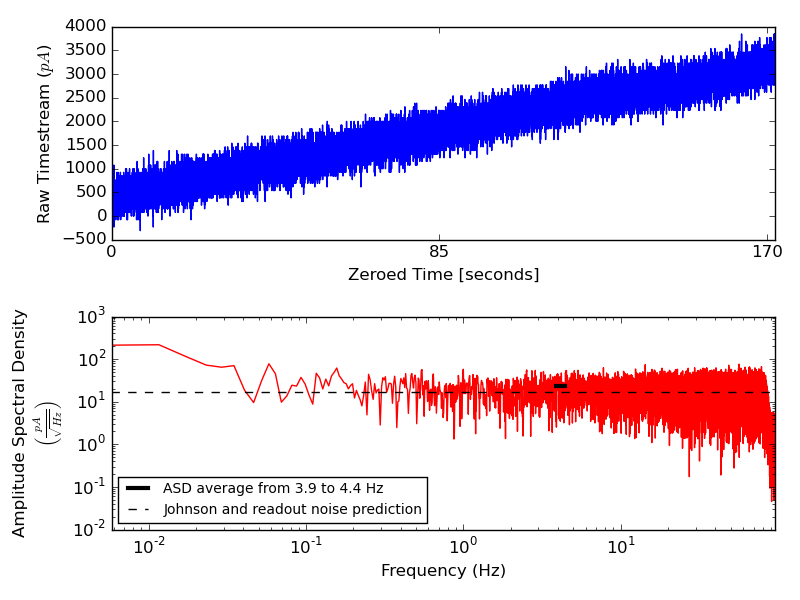
\includegraphics[height=3in]{figures/board64_wire2_ch02_1356968507s_overbias}
%\caption{{\it Top:} Raw overbiased bolometer timestream multiplied by the measured transfer function to convert from \ac{DfMUX} demodulated counts to $pA$. {\it Bottom:} The square root of the \ac{PSD} of the timestream above. The measured white noise level, indicated by the short, thick black line, is taken to be the square root of the average value of the \ac{PSD} from 3.9 to 4.4~Hz. This frequency range is chosen to fall in the polarization band, between half-wave plate harmonics. The overbiased noise prediction, the quadrature sum of the Johnson and readout noise, is indicated by the thin dashed black line. }
%\label{fig:one_bolo_overbias_noise}
%\end{center}
%\end{figure}
%% figure comments (\comred{seconds is in square brackets but other units are in parentheses! bin psd so it is less spiky/foresty? decrease y axis range of psd so it spans 2 (or 3) orders of magnitude instead of 5? Timestream just happened to start at zero. Is that ok? Looks too contrived? did 172 sec chunks for analysis, long enough? probably half-wave plate instead of \ac{HWP} since we're not talking about HWP in this paper? don't mention harmonics (and why you chose 3.9 to 4.4~Hz) at all? or refer to where it is talked about? is it talked about?})
%
%\begin{figure}[ht!]
%\begin{center}
%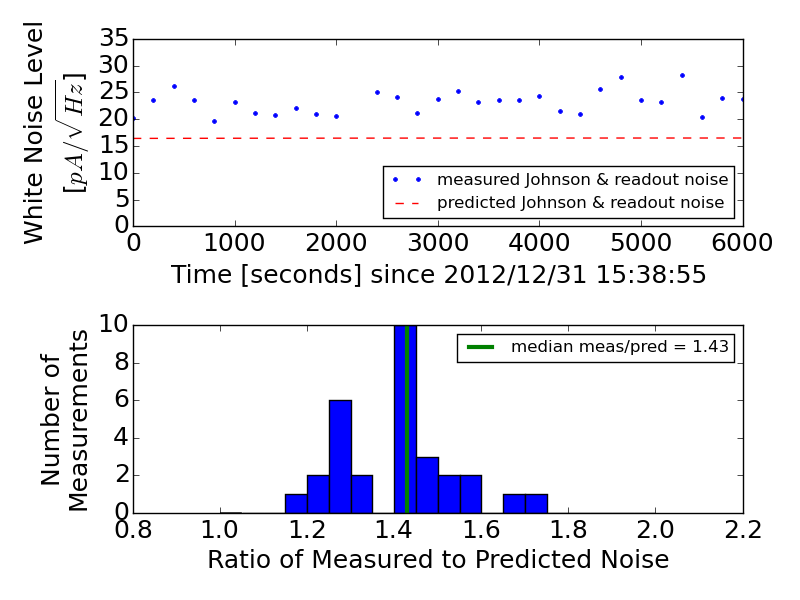
\includegraphics[height=3in]{figures/board64_wire2_ch02_overbias_noise_vs_time}
%\caption{{\it Top:} The predicted and measured overbiased noise, Johnson and readout, for bolometer 250-23-09-09 as a function of time. The prediction is the red horizontal dashed line at 16.4~$pA/\sqrt{Hz}$. Each blue dot is a measurement of the white noise level from the \ac{PSD}. {\it Bottom:} A histogram of the ratio of each measurement to prediction in the timestream above. The median value for this bolometer is 1.43.}
%\label{fig:one_bolo_overbias_noise_vs_time}
%\end{center}
%\end{figure}
%
%\begin{figure}[ht!]
%\begin{center}
%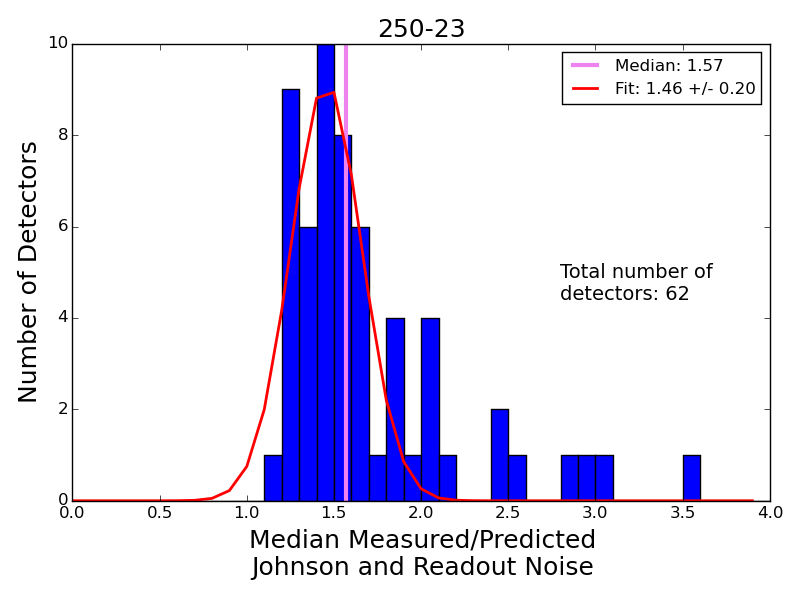
\includegraphics[height=3in]{figures/250-23_overbias_meas_pred_noise_histogram.png}
%\caption{Histogram of the median value of the ratio of measured to predicted noise for each bolometer on wafer~250-23. The median of this histogram 
%%i.e. the median of the medians for wafer~250-23,
%is 1.57, consistent with the Gaussian fit (in red) of $1.46 \pm 0.20$.}
%\label{fig:250-23_overbias_hist}
%\end{center}
%\end{figure}
%
%
%\begin{table}[ht!]
%\begin{center}
%\begin{tabular}{|c|c|c|c|}
%\hline  Wafer & Prediction [$pA/\sqrt{Hz}$]& Ground Overbias Noise Ratio & Flight Overbias Noise Ratio \\
%\hline 150-09 & 12.0 & 1.62 & 1.63 \\
%\hline 150-14 & 10.7 & 1.52 & 1.72 \\
%\hline 150-15 & 10.4 & 1.67 & 2.03 \\
%%\hline 150-20 & Failed & Failed \\
%%\hline 150-24 & 7.0 & 1.57 & Failed \\
%\hline 150-39 & 12.4 & 2.20 & 2.48 \\
%\hline 150-43 & 13.5 & 1.49 & 1.43 \\
%\hline 150-47 & 14.2 & 1.62 & 1.71 \\
%\hline 250-23 & 12.5 & 1.58 & 1.57 \\
%\hline 250-24 & 14.6 & 1.73 & 1.80 \\
%%\hline 250-25 & 1.94 & Failed \\
%\hline 250-29 & 11.8 & 2.41 & 2.12 \\
%%\hline 410-18 & 5.40 & Failed \\
%\hline 410-28 & 17.1 & 1.56 & 1.89 \\
%\hline
%\end{tabular}
%\end{center}
%\caption{The first column is the median overbiased noise prediction for each wafer, in $pA/\sqrt{Hz}$. The predicted overbiased noise for each bolometer is the quadrature sum of its readout and Johnson noise terms of the \ac{NEP}. The ratio of measured to predicted overbiased noise is calculated for each detector on the ground in Antarctica and at float. The median value of each wafer, both on the ground and at float, is reported in the final two columns of the table.}
%\label{overbias_noise_table}
%\end{table}%
%%\comred{you should really have overbias noise for ALL wafers, don't you think? yes. you need to go back and measure overbias noise at a time when ALL wafers are operational. if you don't, you need a good explanation as to why there are not 14 wafers in this table. and how do you explain WHY you did the median of the median?}}
%
%
%
%We predict the in-transition \ac{NEP} in $aW/\sqrt{Hz}$ at the detector. 
%We calculate the theoretical Johnson and readout current noise as described above except we also take into account the factor of excess noise measured with the detector overbiased. 
%We assume the factor of excess remains constant when the detector is in its transition, and for each detector on a wafer, we multiply that detector's theoretical Johnson and readout noise by its wafer's median ratio of overbiased to predicted noise reported in \TAB\ref{overbias_noise_table}. 
%In order to convert from current noise to \ac{NEP} at the detector, we divide the Johnson and readout noise terms by the current responsivity. 
%%In order to report the data in units of power at the detector, the Johnson and readout noise as well as the measured counts from the detector timestream need to be divided by the bolometer current responsivity. 
%The current responsivity is the current response of the bolometer to incident power,
%\begin{equation}
%S_I = -\frac{dI}{dP} = \frac{-\sqrt{2}}{V_{bias}} * \frac{\mathcal{L}}{\mathcal{L} + 1} * \frac{1}{1 + i\omega\tau}
%\label{eq:current_responsivity}
%\end{equation}
%where $V_{bias}$ is the voltage bias across the bolometer, $\mathcal{L}$ is the bolometer loopgain, $\omega$ is the angular frequency of the signal modulation, and $\tau$ is the bolometer time constant~\citep{aubin_thesis}. 
%Assuming the loopgain, $\mathcal{L}$, is high and the time constant factor can be neglected, the current responsivity simplifies to $-\sqrt{2}/V_{bias}$, where $V_{bias}$ is calculated from the \ac{DfMUX} board settings and the transfer function from bias amplitude to voltage across the \ac{TES}. 
%This analysis assumes the loopgain for each detector is high and we address this assumption in Section XXX. 
%
%In order to estimate the photon \ac{NEP} contribution, we take $P_{rad}$ to be the radiative load measured by each detector, Section~\ref{sec:optical_load}. 
%The center and width of the observation frequency bands, $\nu$ and $\Delta \nu$, are from calibration measurements of the \ac{EBEX} spectral response on the ground \citep{Zilic_thesis}. 
%We do not have a measure of the photon correlation noise factor, so we assume it is completely correlated, $\xi=1$, and completely uncorrelated, $\xi=0$, and use these two cases to bracket the noise prediction. 
%In reality, the photon noise correlation factor is probably somewhere in between \cite{}. 
%\comred{You need to go read, and make a point to actually understand this time, what exactly determines how much this term contributes to the \ac{NEP}. Also, if you are indeed going to provide a bracket on the prediction for $\xi=0$ and $\xi=1$, you need to figure out how to display this information (table, plot, banded histogram, pie chart...).}
%
%In order to estimate the phonon \ac{NEP} contribution, we get both the bolometer temperature and the thermal conductance from the dark characterization measurements. 
%We take the bolometer temperature to be $T_{critical}$ from the critical transition temperature measurements. 
%%The average thermal conductance has less uncertainty than the dynamic thermal conductance because the measurement of the average thermal conductance does not require knowledge of the power of the thermal conductivity. 
%Though the phonon \ac{NEP} calculation requires knowledge of the dynamic thermal conductance, the dark characterization measurements performed provide only a measure of the average thermal conductance. 
%In order to get from average to dynamic thermal conductance, we assume the thermal conductivity can be described by a power law of power n, $\kappa = \kappa_{0} T^{n}$.
%We then find the dynamic thermal conductance via the following relation between average and dynamic thermal conductance
%\begin{equation}
%G_{dynamic} = (n+1) \frac{1 - T_{bath}/T_{critical}}{1 - T_{bath}^{n+1}/T_{critical}^{n+1}} \times \overline{G}
%\end{equation}
%where $T_{bath}$ is the temperature of the bath, $T_{critical}$ is the detector's measured critical temperature, and n is the power of the thermal conductivity \citep{mather_appliedoptics_1982}. 
%In order to calculate $\gamma$, the factor accounting for the temperature gradient along the weak link from the TES to the bath, we again need to assume the thermal conductivity takes the form of a power law of power n. 
%Gamma is then
%\begin{equation}
%\gamma = \frac{(n+1)}{(n+2)} \frac{1 - (T_{bath}/T_{critical})^{n+2}}{1 - (T_{bath}/T_{critical})^{n+1}}
%\end{equation}
%where $T_{bath}$ is the temperature of the bath, $T_{critical}$ is the detector's measured critical temperature, and n is the power of the thermal conductivity \citep{mather_appliedoptics_1982}. 
%%\comred{I used the derivations/equations from Hannes' thesis, but he says he follows Mather. Should I cite both of them?}
%$T_{bath}$ is measured by a temperature sensor mounted to the stage and $T_{critical}$ is found during the critical transition temperature measurements.
%We take n to be 2 since thermal conductivity measurements of \ac{EBEX} test flight wafers gave values of 2.2 $\pm$ 0.3, 1.9 $\pm$ 0.2, and 2.1 $\pm$ 0.2 for the 150, 250, and 410 GHz bands respectively \cite{hubmayr_thesis}.
%
%The median predicted in transition \ac{NEP} level for each wafer is reported in \TAB\ref{in_transition_noise_table}. 
%There is a piechart breakdown of each contributor to the predicted \ac{NEP} for one 150~GHz detector towards the beginning of flight in Fig.~\ref{fig:in_transition_psd}. 
%The white noise level is measured exactly as is done in the case of overbiased noise, except the timestream has had the \ac{HWP} template subtracted. 
%Fig.~\ref{fig:in_transition_psd} is the square root of the \ac{PSD} of a 172~second chunk of time with the \ac{HWP} template present (red) and the \ac{HWP} template subtracted (yellow) for detector 150-09-XX-XX. 
%The measured white noise level is the square root of the average of the \ac{PSD} between 3.9 and 4.4~Hz, indicated by the short thick black line, and the \ac{NEP} prediction is calculated as described above, indicated by the thin black dashed line. 
%
%For roughly ten minutes after the detectors were tuned for Observation C, the \ac{HWP} was off. 
%We compare the measured white noise level during this time with the \ac{HWP} stationary to the measured white noise level just after this time, with the \ac{HWP} spinning and the template subtracted timestream data, Fig.~\ref{fig:hwp_on_vs_off}. 
%We expected there to be no difference. 
%begin{figure}[ht!]
%\begin{center}
%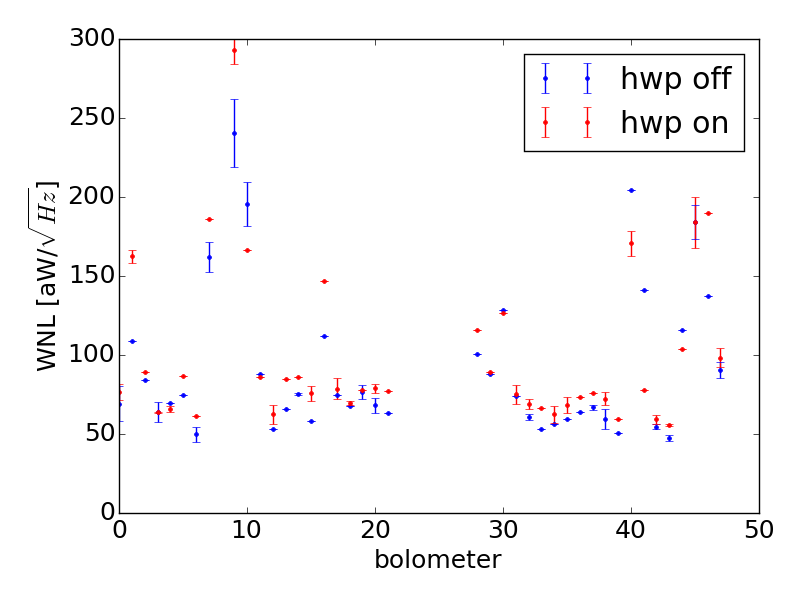
\includegraphics[width=0.4\columnwidth]{figures/hwp_on_and_off_cutoff_at_300aW.png}
%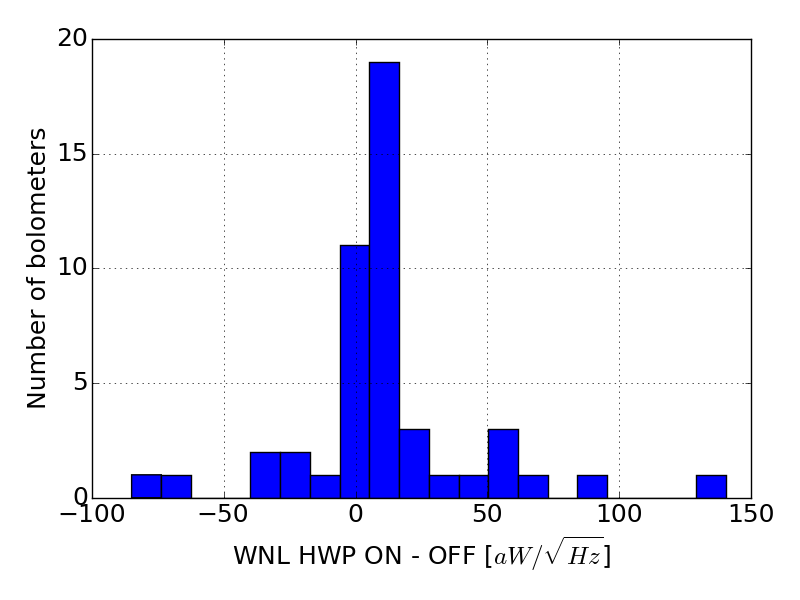
\includegraphics[width=0.4\columnwidth]{figures/hwp_on_and_off_median_diff_histogram.png}
%\caption{{\it Left:} The median \ac{WNL} measured with the \ac{HWP} on (red) and the median \ac{WNL} measured with the \ac{HWP} off (blue). The error bars are the standard deviation of the measurement over ten minutes with the \ac{HWP} off and twenty minutes with \ac{HWP} on. If there was only one chunk of time meeting criteria to perform a \ac{PSD}, the standard deviation is zero and so there is a line through the center of the data point. {\it Right:} A histogram of the median \ac{WNL} measured with the \ac{HWP} on minus the median \ac{WNL} measured with the \ac{HWP} off.}
%\label{fig:hwp_on_vs_off}
%\end{center}
%\end{figure}
%
%
%
%For those detectors which have all of the dark measurements available, throughout flight the noise is calculated and predicted every 172 seconds, provided none of the bolometer timestream data in that chunk has been flagged as bad. 
%The noise, measured and predicted, as a function of time is shown for 150-09-XX-XX in Fig.~\ref{fig:in_transition_noise_vs_time}. 
%%The median value of the ratio of measured to predicted \ac{NEP} for each detector throughout flight is found. 
%The histogram of the median measured to predicted \ac{NEP} for each detector on wafer 150-09 is shown in Fig.~\ref{fig:150-09_median_histogram}.
%Each wafer's median measured to predicted \ac{NEP} ratio is reported \TAB\ref{in_transition_noise_table}. 
%Taking into account the excess overbiased noise and using each detector's measured radiative load, the measured \ac{NEP} agrees with the predictions to within one standard deviation \comred{report gaussian instead of median so it's clear what one sigma is! wait, is this even true for 250 and 410 GHz?! also, update to use the data from every 172 sec (instead of the every 200s data which was missing some bolos)}. 
%
%\subsubsection{Loopgain}
%\label{sec:loopgain}
%
%In order to convert from units of current to power at the detector, these results assume the detectors are operating deep in their transitions. 
%A detector well into its transition has a high loopgain and so $\mathcal{L}/(\mathcal{L} + 1) \sim 1$, and the current responsivity can be approximated as $-\sqrt{2}/V_{bias}$. 
%If, however, the detector is not dropped deep into its transition, then it is not safe to assume the loopgain is high and the factor of  $\mathcal{L}/(\mathcal{L} + 1)$ in the responsivity should not be neglected. 
%%The \ac{EBEX} detectors are dropped to 85\% of their normal resistance for the majority of flight. 
%We can estimate the loopgain at any depth in the transition via the definition of loopgain, 
%\begin{equation}
%\mathcal{L} \equiv \frac{P\alpha}{GT}
%\end{equation}
%where $P$ is the Joule power dissipated in the bolometer, alpha is a unitless number quantifying the temperature sensitivity, $G$ is the dynamic thermal conductance, and $T$ is the bolometer temperature \citep{irwin_book_2005}. 
%The largest uncertainty is in the value of $\alpha$, 
% \begin{equation}
% \alpha \equiv \frac{\partial \log R}{\partial \log T}=\frac{T}{R} \frac{dR}{dT}
% \end{equation}
% where R is the detector resistance and T is the detector temperature \citep{irwin_book_2005}. 
%The \ac{EBEX} detector resistances are known to 10\%, but near the transition, $dR/dT$ changes steeply given small changes in detector resistance. 
%If we take a typical resistance versus temperature curve and overestimate the average value of R by 10\%, then $\mathcal{L}$ decreases by a factor of 2.
%If we underestimate R by 10\%, then $\mathcal{L}$ increases by a factor of 7. 
%%\comred{Provide a quantitative uncertainty on $\alpha$ given the uncertainty on R \& dR/dT.}
%\comred{Given this, can we even report on/conclude anything from the loopgain measurements??}
%
%In order to provide an estimate of the effect of operating the detectors at 85\%, near the top of their transitions, we calculate the loopgain for the detectors on wafer 250-23. 
%The left panel of Fig.~\ref{fig:loopgain_histogram} is a histogram of the calculated loopgains for one tuning of these detectors during flight. 
%When we perform the analysis of the noise performance using the measured loopgains instead of assuming the loopgain is 10000, we find the ratios of measured to predicted noise in the right panel of Fig.~\ref{fig:loopgain_histogram}. 
%The median ratio increases from 1.05 to 1.15. 
%Our final results reported in \TAB\ref{in_transition_noise_table} are a lower limit on the noise performance, and if all wafers behave similarly to wafer~250-23, taking into account the measured loopgain increases the ratio of measured to predicted noise by $\sim$10\%. 
%
%
% %\comred{is referencing the irwin/hilton chapter the right thing to do?}
%%If the resistance values are systematically 10\% too low, then the median loopgain changes from 9 to 7. 
%%If instead the resistance values are systematically 10\% too high, then the median loopgain changes from 9 to 20. 
%
%% would like to include iv curve loopgains as well, BUT I still don't understand how the equation follows from the referenced paper in ziggy's thesis.
%%The loopgain can also be estimated from the iv measurement. 
%%\comred{You need to comment on how safe (or un-safe) it is to make those sweeping assumptions that loopgain is huge and time constant correction factor is neglect-able}
%% do we say in transition or in-transition ? 
%
%\begin{figure}[ht!]
%\begin{center}
%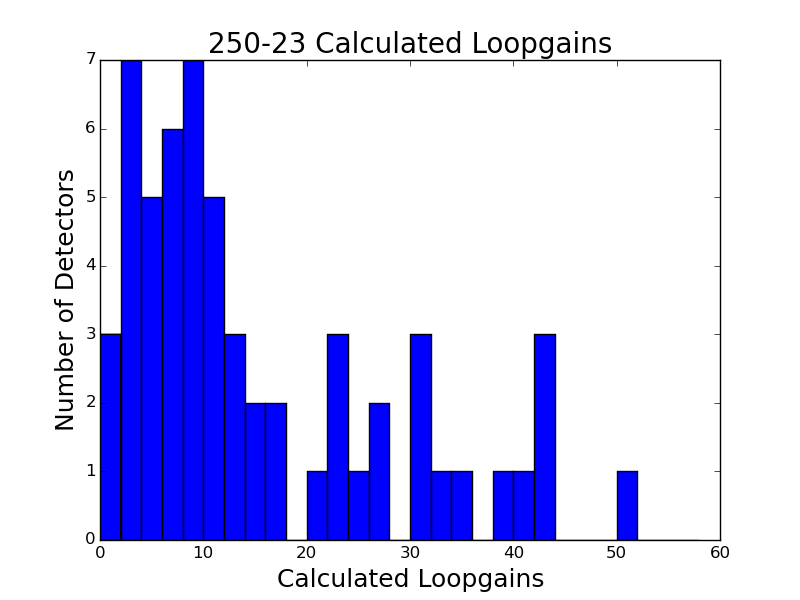
\includegraphics[width=0.4\columnwidth]{figures/250-23_calculated_loopgains_histogram.png}
%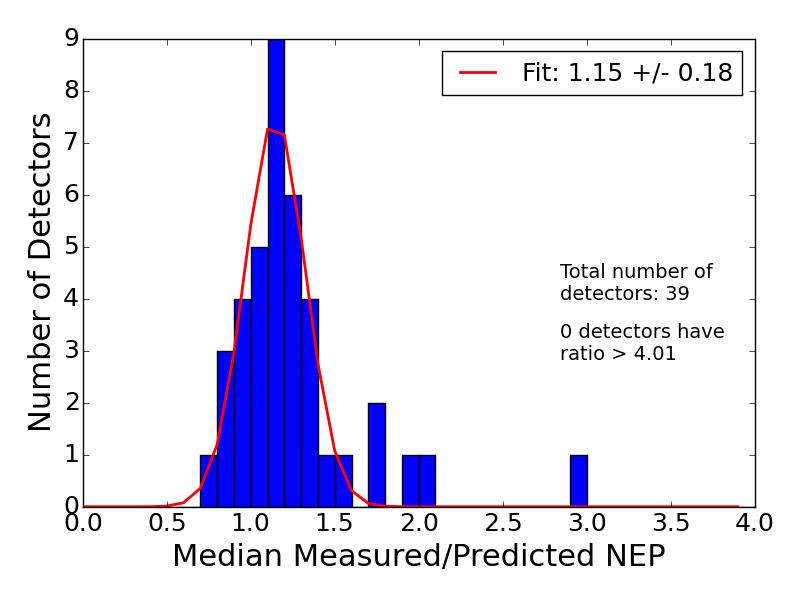
\includegraphics[width=0.4\columnwidth]{figures/250-23_meas_pred_ratios_obsc_calculated_loopgain.png}
%\caption{{\it Left:} The calculated loopgains for wafer 250-23 using Joule power measured from flight iv curves, alpha and temperature from dark resistance versus temperature measurements, and thermal conductance from dark iv curves and assuming the power of thermal conductivity is 2. {\it Right:} The median ratio of measured to predicted \ac{NEP} for each detector on wafer 250-23 using the calculated loopgains instead of assuming the detector is deep in its transition and the loopgain is 10000.}
%\label{fig:loopgain_histogram}
%\end{center}
%\end{figure}
%
%
%
%\begin{figure}[ht!]
%\begin{center}
%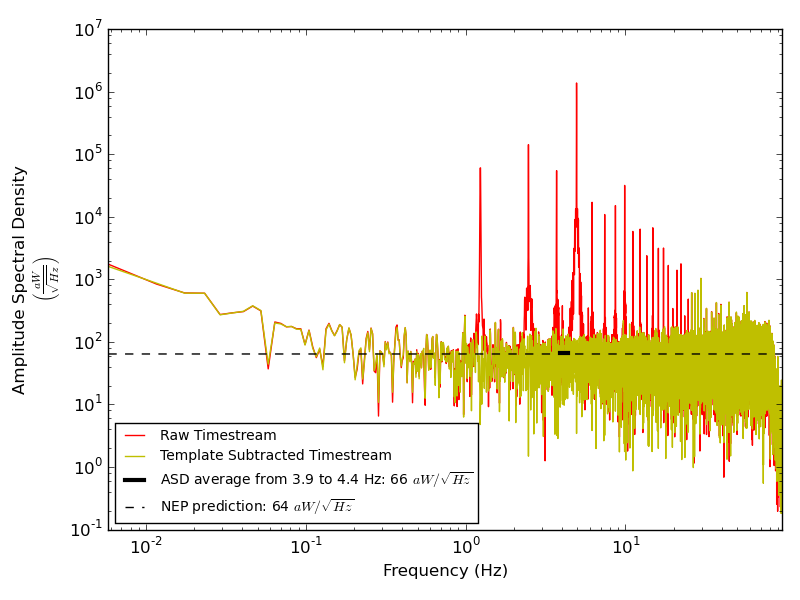
\includegraphics[width=0.69\columnwidth]{figures/board69_wire3_ch11_1356987555s_transition}
%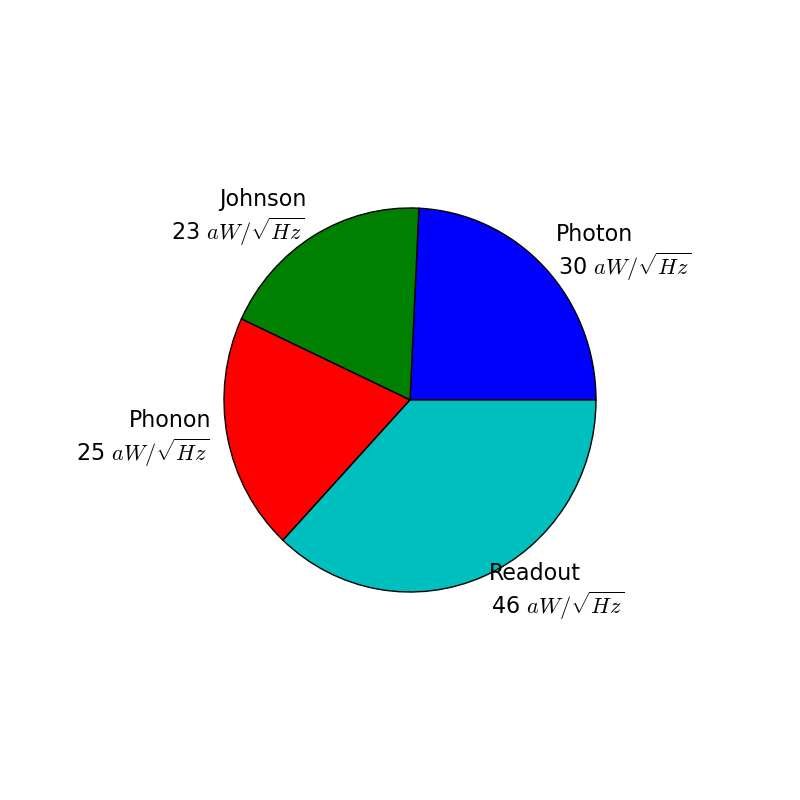
\includegraphics[width=0.29\columnwidth]{figures/board69_wire3_ch11_1356987555s_aW}
%\caption{\comred{This spectrum is whiter than 68-2-04's was, but now the prediction and measurement almost line up and it's difficult to see the measurement line. Also, this bolo maybe isn't good because it is not dominated by photon noise. (why photon noise so small anyhow?) Does y axis span too many orders of magnitude? since this isn't about template subtraction, should we not even show the asd of the raw timestream? if pie chart is useful, maybe make it a subfigure on the asd? If you do use this guy and pie chart, the word readout needs to move right.}}
%\label{fig:in_transition_psd}
%\end{center}
%\end{figure}
%
%\begin{figure}[ht!]
%\begin{center}
%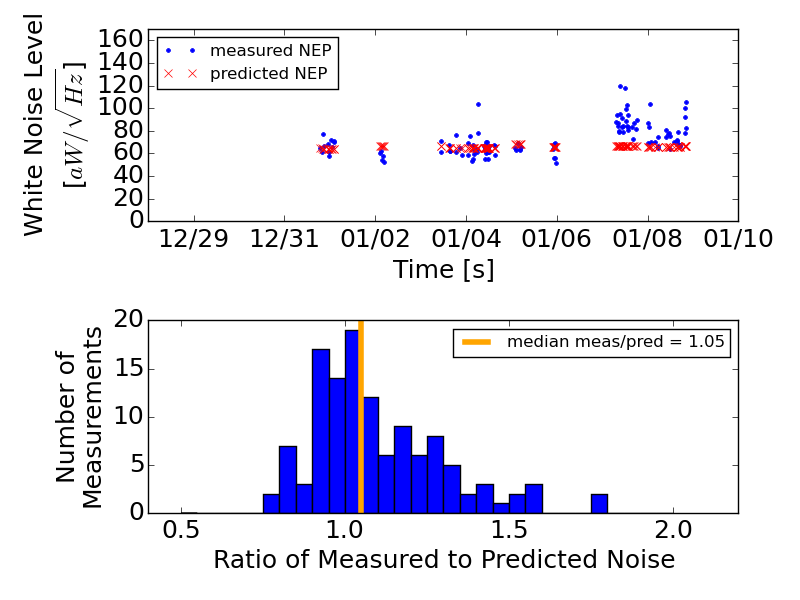
\includegraphics[height=3in]{figures/board69_wire3_ch11_noise_vs_time}
%\caption{\comred{This bolo has median 1.05, much closer to median of wafer 150-09 (1.07), so this should address Matt's confusion. it does seem all bolos on this wafer show increase in optical load on 01/03, decrease on 01/04, and decreased optical load later in flight (e.g 01/07 \& 01/08) when we go deeper in transition. do we prefer a linear or log scale for the y axis?}}
%\label{fig:in_transition_noise_vs_time}
%\end{center}
%\end{figure}
%
%\begin{figure}[ht!]
%\begin{center}
%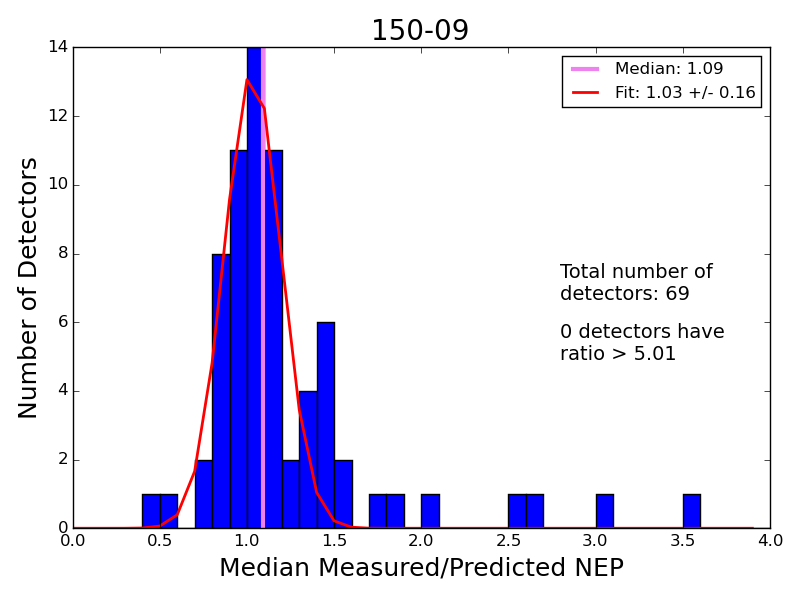
\includegraphics[height=3in]{figures/150-09_NEP_median_meas_pred_distribution}
%\caption{\comred{do you want to keep fit on plot? number of channels and greater than text printed on plot should just be deleted (or can go in caption if need be). Maybe pinkish median line is not a good color for black and white?}}
%\label{fig:150-09_median_histogram}
%\end{center}
%\end{figure}
%
%\begin{table}[ht!]
%\begin{center}
%\begin{tabular}{|c|c|c|c|}
%\hline  Wafer & Predicted NEP [$aW/\sqrt{Hz}$] & Measured/Predicted NEP & Channels \\
%\hline 150-09 & 68.2 & 1.09 & 69 \\
%\hline 150-14 & 44.2 & 0.64 & 12 \\
%\hline 150-15 & 46.7 & 1.12 & 22 \\
%%\hline 150-20 & n/a & 0 \\
%%\hline 150-24 & n/a & 0 \\
%\hline 150-39 & 76.5 & 1.01 & 19 \\
%\hline 150-43 & 53.4 & 1.12 & 51 \\
%\hline 150-47 & 57.9 & 1.46 & 11 \\
%\hline 250-23 & 77.1 & 1.05 & 61 \\
%\hline 250-24 & 73.4 & 1.49 & 51 \\
%%\hline 250-25 & n/a & 0 \\
%\hline 250-29 & 91.3 & 1.39 & 40 \\
%%\hline 410-18 & n/a & 0 \\
%\hline 410-28 & 102 & 2.00 & 68 \\
%\hline
%\end{tabular}
%\end{center}
%\caption{The median predicted \ac{NEP} for each wafer, in $aW/\sqrt{Hz}$, is reported in the second column. The prediction takes into account each wafer's at float overbiased measured to predicted noise ratio, each detector's dark characterization measurements, and each detector's measured radiative load. For each wafer, the median ratio of the measured \ac{NEP} to the predicted \ac{NEP} and the number of detector channels included are reported in the final two columns of the table. \comred{better to report gaussian fit instead of median of medians ???}}
%\label{in_transition_noise_table}
%\end{table}
%
%\begin{figure}[ht!]
%\begin{center}
%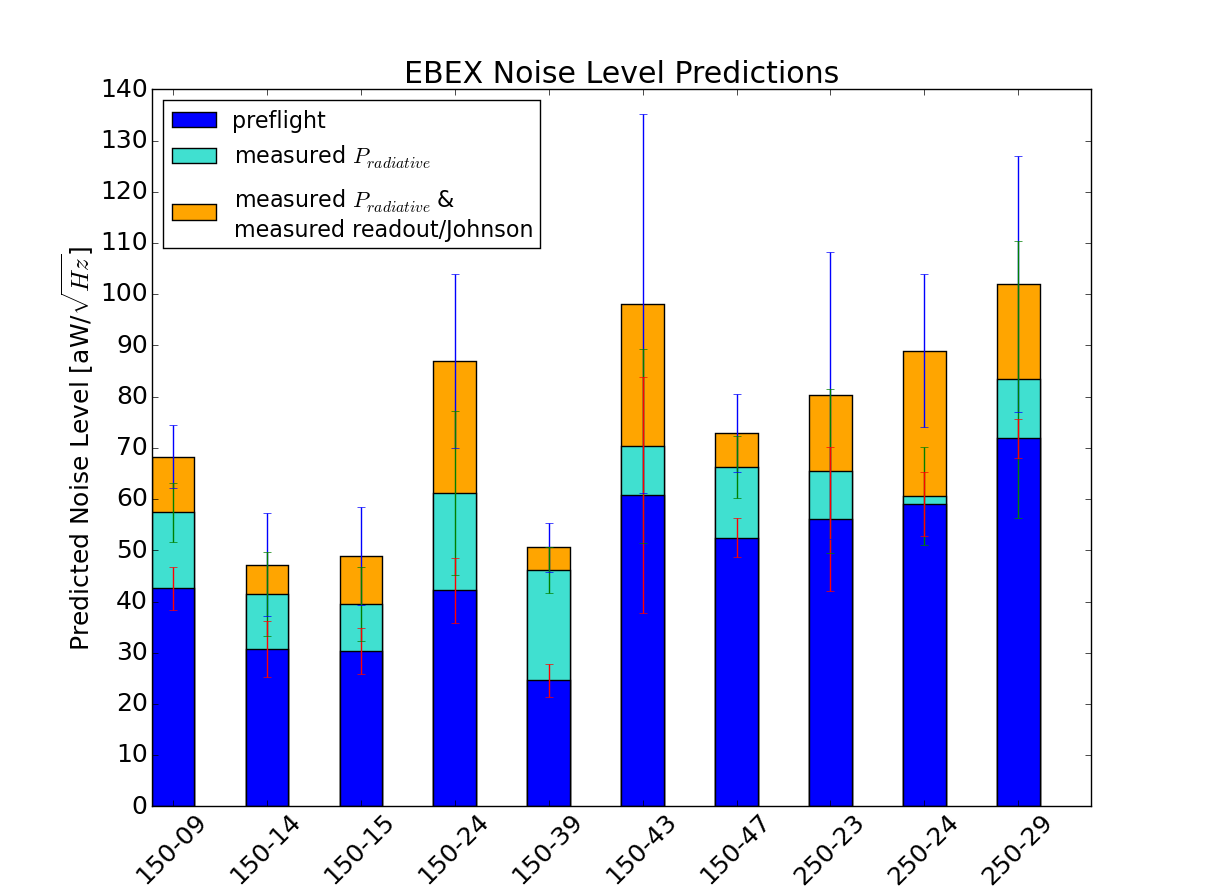
\includegraphics[height=3in]{figures/ebex_noise_level_predictions_barchart_per_wafer}
%\caption{The average \ac{NEP} prediction for each flight wafer. The dark blue bars are the expected noise given the measured detector parameters and the preflight radiative load prediction for each frequency band, the turquoise bars are the additional \ac{NEP} given the radiative measured load at float, and the orange bars are the additional \ac{NEP} from assuming the excess noise measured overbiased is still a constant factor when the detectors are in the transition. The error bars on the blue are the standard deviation of the prediction due to the variation in measured detector parameters, on the turquoise and gold the standard deviation increases due variation in measured radiative loads. \comred{remove std bars ??}}
%\label{fig:nep_prediction_barchart}
%\end{center}
%\end{figure}
%
%
%
%
%
%
%noise at float blah blah blah
%
%\begin{figure}[ht]
%\centering
%   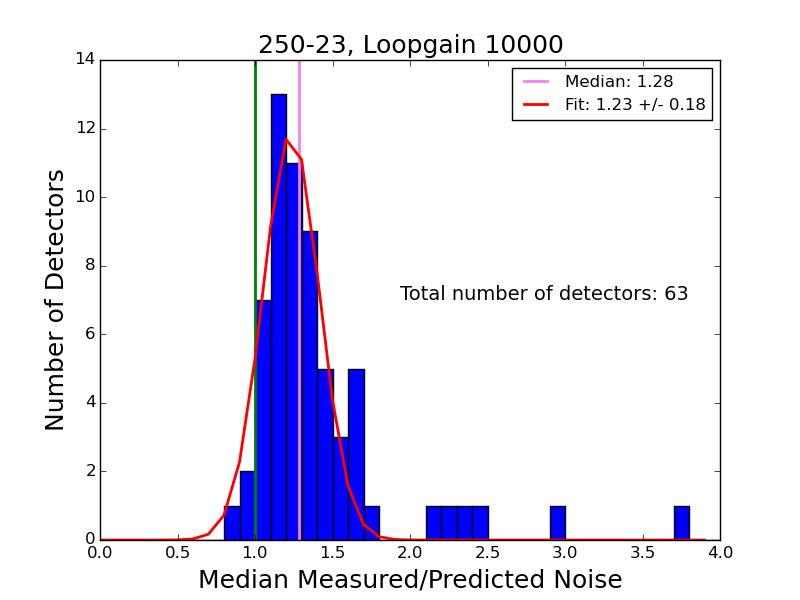
\includegraphics[width=0.33\textwidth]{./figures/250-23_it_meas_pred_ratio_loopgain_10000.png}
%   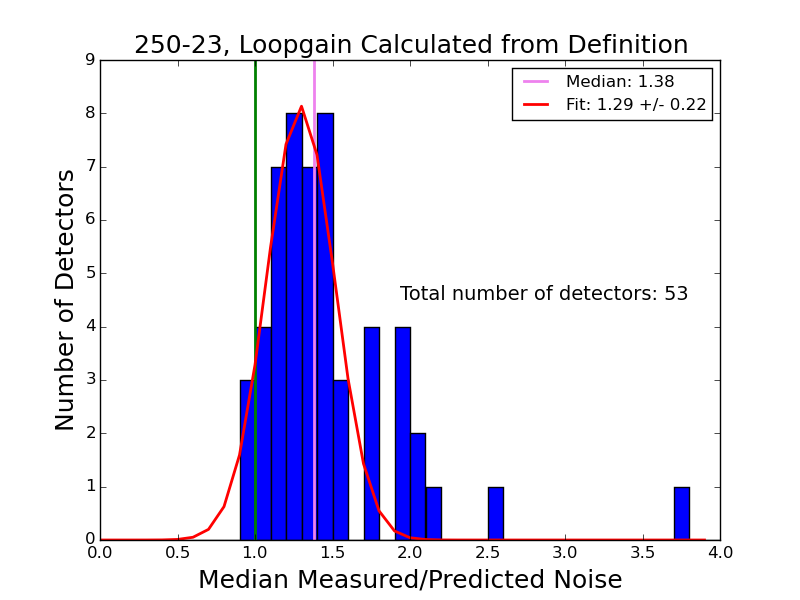
\includegraphics[width=0.33\textwidth]{./figures/250-23_it_meas_pred_ratio_loopgain_calc.png}
%   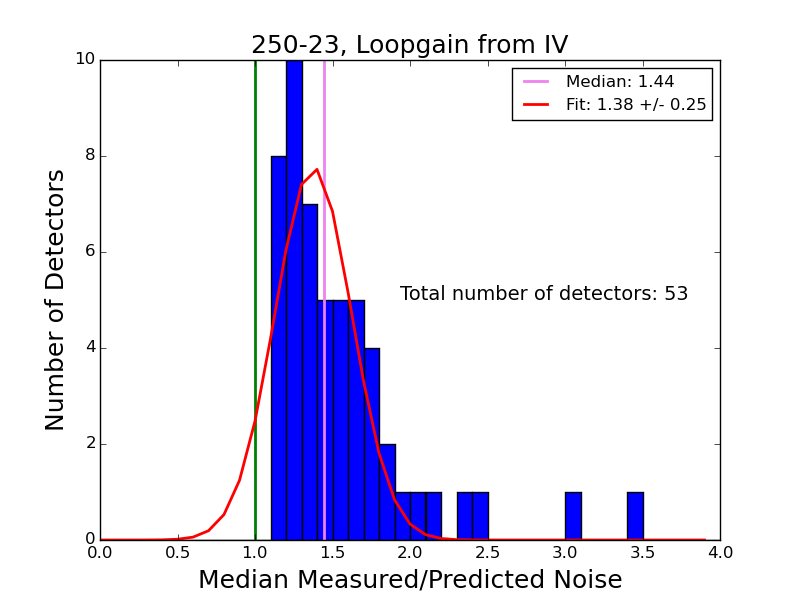
\includegraphics[width=0.33\textwidth]{./figures/250-23_it_meas_pred_ratio_loopgain_iv.png}
%\caption{Wafer 250-23 noise performance for three different loopgain value scenarios. The most optimistic is to assume the detectors are
%                deep in the transition (NEED TO DEFINE THIS) and so the loopgain is huge, $L$=10000 (upper left). If the detectors are not 
%                deep in the transition, we can calculate the loopgain and include it in the conversion from counts to power. The loopgain 
%                can be calculated from its definition (upper right) and can also be estimated from the IV curve (lower).  
%                \label{fig:effect_of_loopgain}}
%\end{figure}
%
%
%%%%%%%%%%%%%%%%%%%%%%%%%%%%%%%%%%%%%%%%%%%%%%%%%%%%%%%%%%%%%%%%%%%%%%%%%%%%%%}}}
